\documentclass[french,11pt,a4paper]{article}

\usepackage[T1]{fontenc}
\usepackage[french]{babel}
% !TeX spellcheck = fr_FR

\title{Probabilité des critères de vote \\ Compte rendu de TIPE}
\author{\textit{Vangi}lluwen Hugo}
\date{26 mai 2024}

\usepackage{geometry}
\geometry{
	a4paper,
	top=2cm,
	bottom=2cm,
	right=2cm,
	left=2cm
}

% Formules mathématiques
\usepackage{amsmath}
\usepackage{amsfonts}
\usepackage{amssymb}
\usepackage{amsthm}
\usepackage{nicefrac}
\usepackage{mathrsfs}

\usepackage{enumitem}

\usepackage{hyperref}
\makeatletter
\hypersetup{
	colorlinks=true,
	linkcolor=blue,
	filecolor=magenta,
	urlcolor=cyan,
	citecolor=olive,
	pdftitle={Compte rendu de TIPE},
	pdfauthor={\@author}
}
\makeatother

% Graphiques
\usepackage{graphicx}
\graphicspath{ {../simulation/figures/}}
\usepackage[linguistics]{forest}
\usepackage{subcaption}
\usepackage{changepage}
\usepackage{float}


% Environnements
\theoremstyle{definition}
\newtheorem{definition}{Définition}
\theoremstyle{plain}
\newtheorem{theoreme}{Théorème}
\newtheorem{proposition}{Proposition}
\theoremstyle{remark}
\newtheorem*{exemple}{Exemple}

% Ensembles usuels en systèmes de votes
\newcommand{\C}{\mathcal{C}}
\newcommand{\V}{\mathcal{V}}
\newcommand{\W}{\mathcal{W}}
\newcommand{\pO}{\mathcal{O}}
\newcommand{\SV}{\mathscr{S}}
\newcommand{\D}{\mathcal{D}_\mathcal{O}}

\newcommand{\propriete}[1]{
	\label{#1}
	\underline{#1} \newline
}


\begin{document}
	\maketitle

	\begin{abstract}
		En théorie du choix social, les systèmes de vote sont évalués par différents critères. Cependant, le respect ou non de ces critères est une information booléenne. C'est pour quoi j'ai cherché une façon plus nuancée d'évaluer les systèmes de vote. Je vais m'intéresser à la probabilité de respecter un certain critère en prenant un profil de préférence au hasard.
	\end{abstract}

	\tableofcontents

	% !TeX root = TIPE_vangi.tex
% !TeX spellcheck = fr

\section{Introduction}

Les systèmes de vote c'est-à-dire les processus qui, à partir de préférences individuelles, donne la préférence collective sont un élément clef des démocraties modernes, permettant de recueillir directement l'avis du peuple. Le choix d'un mode de scrutin est crucial puisqu’il modifie le résultat et, surtout, la façon dont résonnent les électeurs (vote stratégique). Cependant, un tel choix est difficile de part le nombre de critères à vérifier et l'inexistence d'un système de vote parfait (voir le théorème d'Arrow et celui de Gibbard-Satterthwaite). Le respect ou non des critères est booléen. Dans ce TIPE, j'ai cherché un indicateur continu pour classer les systèmes de vote. J'ai étudié la probabilité pour qu'un profil de préférence respecte tel ou tel critère.

Avant de lire ce document, je recommande les trois articles de Rémi Peyre \cite{math_démocratie}.

Nous allons utiliser les notations de Lê Nguyên Hoang \cite{randomized_Condorcet}. Considérons un ensemble fini $\C$ de choix et un ensemble fini $\V$ de votants. Notons $\pO$ l'ensemble des \hyperref[Relation de préordre]{relations de préordre totales} sur $\C$ et $\mathfrak{O}$ l'ensemble des \hyperref[Relation d'ordre]{relations d'ordre totales} sur $\C$.

\begin{definition}
	\underline{Système de vote} \\
	Soit $\D \in \mathcal{P}(\pO)$. Une fonction notée $\SV$ de ${\D}^\V$ dans $\pO$ est un système de vote dont $\D$ est le domaine de vote (qui indique la forme que devront prendre les bulletins).
	\begin{equation}
		\SV : {\D}^\V \rightarrow \pO
	\end{equation}
	Remarquons que le système peut être restreint à ${\D'}^\V$ que l'on notera $\SV_{|\D'}$. Par exemple, $\mathscr{S}_{|\mathfrak{O}}$. \\
	Un élément de ${\D}^\V$ est appelé profil de préférence et représente les bulletins de chaque électeur distinctement.
\end{definition}

	% !TeX root = TIPE_vangi.tex
% !TeX spellcheck = fr

\section{Relations de préordre}

\subsection{Définitions générales}

\begin{definition}
	\propriete{Relation de préordre}
	Une relation de préordre ou simplement préordre $\theta$ ou $\succ_\theta$ sur $E$ est un relation binaire :
	\begin{itemize}
		\item \textbf{réflexive} : $\forall x \in E, x \succ_\theta x$
		\item \textbf{transitive} : $\forall (x, y, z) \in E^3, [x \succ_\theta y \wedge y \succ_\theta z] \implies x \succ_\theta z$
	\end{itemize}
	Elle est dite \textbf{totale} si $\forall (x, y) \in E^2, x \succ_\theta y \vee y \succ_\theta x \vee x = y$.
\end{definition}

Notons $\pO$ l'ensemble des préordres totaux sur $\C$.
Une relation de préordre est représenté par l'ensemble des candidats ordonnés et séparé par ">" ou "=".

\begin{exemple}
	A > D = C > B
\end{exemple}

\begin{definition}
	\propriete{Relation d'ordre}
	Une relation d'ordre $\theta$ sur $E$ est un relation de préordre :
	\begin{itemize}
		\item \textbf{antisymétrique} : $\forall (x, y) \in E^2, [x \succ_\theta y \wedge y \succ_\theta x] \implies x = y$
	\end{itemize}
\end{definition}


Notons $\mathfrak{O}$ l'ensemble de relations d'ordre totales sur $\C$. Leur représentation ne contient aucun "=".

\begin{exemple}
	 D > B > C > A
\end{exemple}

\begin{definition}
	\propriete{Relation d'équivalence}
	Une relation d'ordre $\theta$ sur $E$ est un relation de préordre :
	\begin{itemize}
		\item \textbf{symétrique} : $\forall (x, y) \in E^2, x \succ_\theta y \implies y \succ_\theta x$
	\end{itemize}
\end{definition}


\subsection{Relations induites}

\begin{definition}
	\propriete{majorants et minorants}
	Soit $\theta \in \pO$ et $E \in \mathcal{P}(\C)$.
	\begin{equation*}
		M_\theta (E) = \left\{ x \in \C \;|\; \forall y \in \C, x \succ_\theta y \right\}
	\end{equation*}
	\begin{equation*}
		m_\theta (E) = \left\{ x \in \C \;|\; \forall y \in \C, y \succ_\theta x \right\}
	\end{equation*}
\end{definition}

\begin{proposition}
	Si $E$ n'est pas vide, les majorants et les minorants ne le sont pas non plus.
\end{proposition}

\begin{proposition}
	Pour une relation d'ordre totale, les deux ensembles ci-dessus sont des singletons.
\end{proposition}

\begin{definition}
	\propriete{Relation de pseudo-égalité}
	Soit $\theta \in \pO$. Soient $(x, y) \in \C^2$.
	\begin{equation}
		x \asymp_\theta y \iff x \succ_\theta y \wedge y \succ_\theta x
	\end{equation}
	$\asymp_\theta$ est une relation d'équivalence.
\end{definition}

\begin{proof}
	~\newline
	\begin{itemize}
		\item \textit{Réflexivité} Soit $x \in \C$. Par réflexivité de $\theta$, $x \succ_\theta x$ donc $x \asymp_\theta x$.
		\item \textit{Transitivité} Soit $(x, y, z) \in \C^3$ tel que $x \asymp_\theta y$ et $y \asymp_\theta z$.
		Alors $x \succ_\theta y$ et $y \succ_\theta z$ donc $x \succ_\theta z$.
		De même, $y \succ_\theta x$ et $z \succ_\theta x$ donc $z \succ_\theta x$.
		D'où $x \asymp_\theta z$.
		\item \textit{Symétrie} $\wedge$ est commutatif.
	\end{itemize}
\end{proof}

\begin{theoreme}
	Soit $\theta \in \pO$ et $E \in \mathcal{P}(\C)$.
	\begin{equation*}
		\max_\theta E \in \nicefrac{\C}{\asymp_\theta}
		\quad \wedge \quad
		\min_\theta E \in \nicefrac{\C}{\asymp_\theta}
	\end{equation*}
\end{theoreme}

\begin{proof}
	Traitons $\max$. La démonstration pour $\min$ est sensiblement la même. \\
	Soit $(x, y) \in \left(\max_\theta E\right)^2$. Par définition de $\max$, comme $x \in \max_\theta E$ et $y \in \C$, $x \succ_\theta y$. De même, $y \succ_\theta x$. Ainsi $\forall (x, y) \in \left(\max_\theta E\right)^2, x \asymp_\theta y$.
\end{proof}

\begin{definition}
	Le théorème précédent nous permet de définir l'application $\varXi_\theta$ pour $\theta \in \pO$ :
	\begin{equation}
		\varXi_\theta \
		\left| \ \begin{matrix}
			\mathcal{P}(\C) &\rightarrow& \underset{n = 0}{\overset{|\C|}{\bigcup}} \left(\nicefrac{\C}{\asymp_\theta}\right)^n \\
			~\\
			E &\mapsto& \left\{ \begin{matrix}
				\emptyset &\text{si }& E = \emptyset \\
				\left(\displaystyle \max_\theta E, \ \varXi_\theta\left(E \setminus \max_\theta E\right) \right) &\text{si }& E \neq \emptyset
			\end{matrix} \right.
		\end{matrix} \right.
	\end{equation}
	Avec, pour tout ensemble $E$, $E^0 = \emptyset$.
\end{definition}

\begin{exemple}
	Pour $\C = \{A, B, C, D, E\}$ et $\theta = D > B = C = E > A$,
	$\varXi(\C) = (\{D\}, \{B,C,E\}, \{A\})$
\end{exemple}

\begin{proposition}
	\begin{equation*}
		\forall \theta \in \pO, \
		\forall E \in \mathcal{P}(\C), \
		\varXi_\theta(E) \in \left(\nicefrac{\C}{\asymp_\theta}\right) ^ {\left|\nicefrac{E}{\asymp_\theta}\right|}
	\end{equation*}
	Visuellement, $\left| \varXi_\theta(\C) \right|$ est égal au nombre de '>' plus 1 dans la représentation de $\theta$.
\end{proposition}

\begin{proof}
	Récurrence sur le cardinal de $E$.
\end{proof}

\begin{proposition}
	$\varXi_\theta(E)$ forme une partition de $E$.
\end{proposition}

\begin{proof}
	Récurrence sur le cardinal de $E$.
\end{proof}


\begin{definition}
	\underline{Relation induite sur les parties de $\C$} \\
	Soit $\theta \in \pO$. Soient $(E, F) \in \mathcal{P}(\C)^2$. \\
	Sous réserve de non-vacuité, soient $x \in \max_\theta E \setminus (E \cap F)$ et $y \in \max_\theta F \setminus (E \cap F)$ quelconques.
	\begin{equation}
		E \succ_\theta F \iff
		\left\{ \begin{matrix}
			Vrai &si \ F = \emptyset \\
			Faux &si \ E = \emptyset \ et \ F \neq \emptyset \\
			x \succ_\theta y &si \ x \not \asymp_\theta y \\
			E \!\setminus\! \{x\} \succ_\theta F \!\setminus\! \{y\} &si \ x \asymp_\theta y
		\end{matrix} \right.
	\end{equation}
\end{definition}

\begin{proposition}
	Cette relation induite est un préordre.
\end{proposition}

\begin{proof}
	Vérifions que cette relation est bien définie c'est-à-dire qu'elle ne dépend pas des éléments $x$ et $y$ choisis.
	Soient $(x, x') \in \left( \max_\theta E \setminus (E \cap F) \right)^2$ et $(y, y') \in \left( \max_\theta F \setminus (E \cap F) \right)^2$.
	
	Supposons $x \not \asymp_\theta y$. Alors $x' \not \asymp_\theta y'$.
	Montrons que $x \succ_\theta y \iff x' \succ_\theta y'$.
	Sachant que $x' \succ_\theta x$ et $y \succ_\theta y'$, par transitivité, $x \succ_\theta y \implies x' \succ_\theta y'$.
	Sachant que $x \succ_\theta x'$ et $y' \succ_\theta y$, par transitivité, $x' \succ_\theta y' \implies x \succ_\theta y$. D'où l'indépendance aux éléments $x$ et $y$ choisis si $x \not \asymp_\theta y$.
	
	Supposons $x \asymp_\theta y$. Alors $x' \asymp_\theta y'$. Ainsi, par récurrence immédiate, à force d'enlever des éléments de E et de F, soit l'un des deux devient vide soit $x \not \asymp_\theta y$.
	C'est-à-dire que l'on retombe sur l'un des trois autres cas qui sont eux-mêmes indépendants des $x$ et $y$ choisis. Donc cette définition est indépendantes des éléments $x$ et $y$ choisis. Donc la relation induite sur les ensembles est bien définie.
	
	Soit $E \in \mathcal{P}(\C)$. Vérifions que $E \succ_\theta E$. Les ensembles dont on prend les maximum sont égaux. Ainsi, on applique récursivement le quatrième cas, jusqu'à que $E$ soit vide. Donc $E \succ_\theta E$ est vrai. Donc la relation induite est réflexive.
	
	Soient $(E, F, G) \in \mathcal{P}(\C)^3$ tels que $E \succ_\theta F$ et $F \succ_\theta G$. Transitivité à faire.
\end{proof}

\begin{definition}
	\underline{Relation induite sur les préordres sur $\C$} \\
	Soit $\theta \in \pO$. Soient $(\iota, \kappa) \in \pO^2$.
	\begin{equation}
		\iota \succ_\theta \kappa \iff
		\left\{ \begin{matrix}
			Vrai &si \ C = \emptyset \\
			M_\iota(\C) \succ_\theta M_\kappa(\C) &si \ M_\iota(\C) \neq M_\kappa(\C) \\
			\iota_{|\C \setminus M_\iota(\C)} \succ_\theta \kappa_{|C \setminus M_\kappa(\C)} &si \ M_\iota(\C) = M_\kappa(\C)
		\end{matrix} \right.
	\end{equation}
	Cette relation permet donc de classer les résultats des systèmes de vote pour différents profils de préférence du point de vue d'un électeur fixé.
\end{definition}

\begin{proposition}
	Cette relation induite est un préordre.
\end{proposition}

\begin{proof}
	J'ai vraiment la flemme de faire cette démonstration.
\end{proof}


\subsection{Relations de permutation}

\begin{definition}
	\propriete{Relation de permutation sur les familles}
	Soient $E$ et $F$ deux ensembles quelconques.
	\begin{equation}
		\forall \left(x,y\right) \in \left(E^F\right)^2\!, \;
		x \sim y \iff
		\exists \sigma \in \mathfrak{S}_F : x = \left(y_{\sigma(f)}\right)_{f \in F}
	\end{equation}
	Où $\mathfrak{S}_F$ est l'ensemble des permutations de $F$. \\
\end{definition}

\begin{proposition}
	Cette relation est une relation d'équivalence. \\
	Notons $S$ un système de représentant de $\nicefrac{{\D}^\V}{\sim}$.
\end{proposition}

\begin{proof}
	~\newline
	\begin{itemize}
		\item \textit{Réflexivité} Soit $x \in E^F$. $Id_F$ est une permutation de $F$ donc $x \sim x$.
		\item \textit{Transitivité} Soient $(x, y, z) \in \left(E^F\right)^3$ tels que $x \sim y$ et $y \sim z$.
		Fixons $\sigma$ la permutation liant $x$ et $y$ et $\sigma'$ celle liant $y$ et $z$.
		Alors $x = \left(y_{\sigma(f)}\right)_{f \in F} = \left(z_{\sigma \circ \sigma'(f)}\right)_{f \in F}$.
		Or $\sigma \circ \sigma'$ est une permutation donc $x \sim z$.
		\item \textit{Symétrie} Soient $(x, y) \in \left(E^F\right)^2$ tels que $x \sim y$.
		Fixons $\sigma$ liant $x$ et $y$. Alors $\left(x_{Id_F(f)}\right)_{f \in F} = \left(y_{\sigma(f)}\right)_{f \in F}$.
		$\sigma^{-1}$ existe et est une permutation. D'où $\left(x_{\sigma^{-1}(f)}\right)_{f \in F} = \left(y_{Id_F(f)}\right)_{f \in F}$. Donc $y \sim x$.
	\end{itemize}
\end{proof}

\begin{definition}
	\propriete{Relation de permutation sur les préordres}
	\begin{equation}
		\forall (\theta, \iota) \in \pO^2\!, \
		\theta \sim \iota \iff
		\big[ \
			\left|\nicefrac{\C}{\asymp_\theta}\right| = \left|\nicefrac{\C}{\asymp_\iota}\right|
			\ \wedge \
			\varXi_\theta(\C) \sim \varXi_\iota(\C)
		\ \big]
	\end{equation}
\end{definition}

\begin{proposition}
	Cette relation est une relation d'équivalence.
\end{proposition}

\begin{proof}
	Si $\left|\nicefrac{\C}{\asymp_\theta}\right| = \left|\nicefrac{\C}{\asymp_\iota}\right|$, $\varXi_\theta(\C)$ et $\varXi_\iota(\C)$ peuvent bien être comparé avec $\sim$ car ils appartiennent à la même famille ($\left(\nicefrac{\C}{\asymp_\theta}\right)^{\left|\nicefrac{E}{\asymp_\theta}\right|}$. Sinon, ils n'ont pas à être comparé. Donc $\sim$ est bien définie.
	
	$=$ et $\sim$ (sur les familles) sont des relations d'équivalence donc $\sim$ (sur les préordres) en est une aussi.
\end{proof}

\begin{proposition}
	$\nicefrac{\mathfrak{O}}{\sim} = \{\mathfrak{O}\}$
\end{proposition}

\begin{proof}
	Cela revient à montrer que toutes les relations d'ordres sont en relation par $\sim$.
	
	Commençons par montrer que $\forall \theta \in \mathfrak{O}, \nicefrac{\C}{\asymp_\theta} = \C$.
	Soit $\theta \in \mathfrak{O}$. Soit $(A, B) \in \C^2$ tels que $A \neq B$.
	Si $A \asymp_\theta B$ alors, par antisymétrie de $\theta$, $A = B$ ce qui est impossible.
	Donc $A \not \asymp_\theta B$. Ainsi chaque classe d'équivalence ne contiennent qu'un seul élément.
	Or les classes d'équivalence forment une partition de de $\C$. Donc $\nicefrac{\C}{\asymp_\theta} = \C$.
	
	Soit $(\theta, \iota) \in \mathfrak{O}^2$.
	Nous avons $\left|\nicefrac{\C}{\asymp_\theta}\right| = \left|\C\right| = \left|\nicefrac{\C}{\asymp_\iota}\right|$.
	D'après la proposition 3 et le calcul ci-dessus, la relation $\varXi_\theta(\C) \sim \varXi_\iota(\C)$ a un sens dans la famille $\C^{\left|\C\right|}$.
	Posons l'application $\sigma : \C \rightarrow \C$ définie par $\forall k \in [\![1;|\C|]\!], \forall (A, B) \in \varXi_\theta(\C)_k \times \varXi_\iota(\C)_k, \ \sigma(A) = B$.
	$\varXi_\iota(\C)_k$ est un singleton donc $\sigma$ est bien définie.
	D'après la proposition 4, $\varXi_\iota(\C)$ est une partition de $\C$ donc $\sigma$ est surjective.
	D'après l'accident du cardinal fini, $\sigma$ est bijective.
	Ainsi $\theta \sim \iota$.
\end{proof}

\begin{proposition}
	La \hyperref[Relation de permutation sur les préordres]{relation de permutation sur les préordres} peut être vue comme une permutation des choix.
	\begin{equation}
		\forall (\theta, \iota) \in \pO^2, \;
		\theta \sim \iota \iff
		\exists \sigma \in \mathfrak{S}_\C : \forall (A, B) \in \C^2,
		\left[ A \succ_\theta B \!\iff\! \sigma(A) \succ_\iota \sigma(B) \right]
	\end{equation}
\end{proposition}

\begin{exemple}
	$(A > D > B = C > E) \sim (C > E > B = D > A)$
\end{exemple}

\begin{proof}
	À faire
\end{proof}

%\begin{definition}
%	\propriete{Relation de permutation sur les familles de préordres}
%	\begin{equation}
%		\begin{gathered}
%			\forall (\theta, \iota) \in \left(\pO^E\right)^2, \;
%			\theta \sim_\pO \iota \iff \\
%			\exists \sigma \in \mathcal{S}_\C : \forall e \in E, \forall (A, B) \in \C^2,
%			\left[ A \succ_{\theta_e} B \!\iff\! \sigma(A) \succ_{\iota_e} \sigma(B) \right]
%		\end{gathered}
%	\end{equation}
%\end{definition}

	% !TeX root = TIPE_vangi.tex
% !TeX spellcheck = fr

\section{Probabilité des critères}

\subsection{Calcul d'une probabilité d'un critère}

John R. Chamberlin et Michael D. Cohen \cite{spatial_model} ont étudié plusieurs systèmes pour déterminer la probabilité d'élire le vainqueur de Condorcet sous réserve d'existence en utilisant une distribution spatiale des choix et des électeurs. Nous allons maintenant utiliser la culture de l'impartialité (nommé ainsi par ces deux auteurs) pour étendre ce calcul probabiliste à d'autres critères que celui de Condorcet.

\begin{definition}
	Soient $\V$ et $\W$ deux ensembles de votants disjoints et $\mathcal{R}$ un \textit{critère de vote} c'est-à-dire une relation binaire définie sur ${\D}^\V \times {\D}^\W$.
	\begin{equation}
		P_\mathcal{R} (\V, \W)
		= \mathbb{P}_{\theta \sim \mathcal{U}({\D}^\V), \iota \sim \mathcal{U}({\D}^\W)}
		\big[ \theta \; \mathcal{R} \; \iota \big]
	\end{equation}
	Où $\mathcal{U}(E)$ est la distribution uniforme sur  $E$. \\
\end{definition}

\noindent $\mathcal{R}$ est dite impartiale si, pour tous couples $(\theta, \iota) \in {\D}^\V \times {\D}^\W$ et $(\theta', \iota') \in {\D}^\V \times {\D}^\W$,
\begin{enumerate}[label=$(\roman*)$]
	\item permuter les préférences entre $\theta$ et $\theta'$ n'influence pas $\theta \sim \theta' \implies \left[ \theta \mathcal{R} \iota \iff \theta' \mathcal{R} \iota \right]$
	\item permuter les préférences entre $\iota$ et $\iota'$ n'influence pas $\iota \sim \iota' \implies \left[ \theta \mathcal{R} \iota \iff \theta \mathcal{R} \iota' \right]$
	\item permuter les choix de $\C$ n'influence pas
	%			$\begin{gathered}
		%				\forall \sigma \in \mathcal{S}_\C, \forall (A, B) \in \C^2, \\
		%				\left[ \forall v \in \V, A \succ_{\theta_v} B \!\iff\! \sigma(A) \succ_{\theta'_v} \sigma(B) \right]
		%				\wedge \left[ \forall w \in \W, A \succ_{\iota_w} B \!\iff\! \sigma(A) \succ_{\iota_w} \sigma(B) \right] \\
		%				\implies \left[ \theta \mathcal{R} \iota \iff \theta' \mathcal{R} \iota' \right]
		%			\end{gathered}$
\end{enumerate}

\noindent De même, un système de vote est impartial :
\begin{itemize}
	\item pour les votants si le résultat est invariant par permutation des votants
	\item pour les choix si le résultat est invariant par permutation des choix
	\item tout court si il est impartial pour les votants et pour les choix
\end{itemize}


\subsection{Critères impersonnels}

Un critère de vote est dit impersonnel si il est défini pour $\W = \emptyset$ (avec la convention que, pour un ensemble quelconque $E$, nous avons $E^\emptyset = \{\emptyset\}$).

\begin{theoreme}
	\propriete{impersonnel d'invariance par impartialité}
	Si $\mathcal{R}$ est impartiale alors,
	en notant $S$ un système de représentant de $\nicefrac{{\D}^\V}{\sim}$,
	\begin{equation}
		P_\mathcal{R} (\V, \emptyset) =
		\frac{1}{ \left|\D\right| ^ {\left|\V\right|} }
		\sum_{\theta \in S} \left|\bar{\theta}\right|
		\left(
		\left\{\begin{matrix}
			1 &\text{ si } \theta \;\mathcal{R}\; \emptyset \\
			0 &\text{ sinon}
		\end{matrix}\right.
		\right)
	\end{equation}
	Cela permet de réduire grandement le nombre de calcul à effectuer.
\end{theoreme}

\begin{proof}
	Adapter la démonstration de \hyperref[individuel d'invariance par impartialité]{la version individuel du théorème} sachant que $\nicefrac{{\D}^\emptyset}{\sim} = \{\emptyset\}$.
\end{proof}

\begin{definition}
	\propriete{Critère de Condorcet}
	Si il existe un vainqueur de Condorcet alors le système de vote devrait l'élire. L'unicité du gagnant de Condorcet n'est vrai que pour $\D = \mathfrak{O}$. \\
	Posons l'ensemble des vainqueurs de Condorcet $VC$.
	\begin{equation*}
		VC = \left\{ \
			x \in \C \; | \;
			\forall y \in \C, \
			\left|\left\{ v \in \V \;|\; x \succ_{\theta_v} y \right\}\right|
			\geqslant \left|\left\{ v \in \V \;|\; y \succ_{\theta_v} x \right\}\right|
		\ \right\}
	\end{equation*}
	Le critère de Condorcet est défini ainsi :
	\begin{equation}
		\theta \text{ Condorcet } \emptyset \iff
		VC = \emptyset
		\ \vee \
		VC \cap M_{\SV(\theta)}(\C) \neq \emptyset
	\end{equation}
	Ce qui est équivalent à $VC \cap M_{\SV(\theta)}(\C) = \emptyset \implies VC = \emptyset$.
\end{definition}

\begin{definition}
	\propriete{Critère d'unicité du vainqueur}
	Ce critère indique si le vainqueur est unique.
	\begin{equation}
		\theta \text{ UV } \emptyset
		\iff
		\left| M_{\SV(\theta)}(\C) \right| = 1
	\end{equation}
\end{definition}

\subsection{Critères individuels}

Un critère de vote est dit individuel si il est défini pour un singleton $\W = \{w\}$ (avec la convention que, pour un ensemble quelconque $E$, nous avons $E^{\{w\}} = E$).

\begin{theoreme}
	\propriete{individuel d'invariance par impartialité}
	Si $\mathcal{R}$ est impartiale alors,
	en notant $S$ un système de représentant de $\nicefrac{{\D}^\V}{\sim}$ et $T$ un système de représentant  $\nicefrac{\D}{\sim}$,
	\begin{equation}
		P_\mathcal{R} (\V, \{w\}) =
		\frac{1}{ \left|\D\right| ^ {\left|\V\right| + 1} }
		\sum_{\theta \in S} \left|\bar{\theta}\right|
		\left(
		 \sum_{\iota \in T}
		\left\{\begin{matrix}
			\left|\bar{\iota}\right| &\text{ si } \theta \;\mathcal{R}\; \iota \\
			0 &\text{ sinon}
		\end{matrix}\right.
		\right)
	\end{equation}
	Cela permet de réduire grandement le nombre de calcul à effectuer.
\end{theoreme}

\begin{proof}
	Comme $\theta$ et $\iota$ suivent des lois uniforme, la probabilité est le nombre de cas où $\theta \mathcal{R} \iota$ est divisé par le nombre total de cas.
	\begin{equation*}
		P_\mathcal{R} (\V, \{w\}) =
		\frac{ \left| \left\{
			(\theta, \iota) \in {\D}^\V \times \D
			\;|\; \theta \;\mathcal{R}\; \iota
		\right\} \right| }{ \left|
			{\D}^\V \times \D
		\right| }
	\end{equation*}
	Nous remarquons que $\left| {\D}^\V \times \D \right| = \left|\D\right| ^ {\left|\V\right| + 1}$. \\
	Utilisons l’impartialité de $\mathcal{R}$ pour décrire l'ensemble au numérateur en un union disjointe.
	Sachant que ${\D}^\V$ est invariant pour toute permutations des choix, $(iii)$ permet de rassembler les éléments de $\D$.
	\begin{equation*}
		\left\{ (\theta, \iota) \in {\D}^\V \times \D \;|\; \theta \;\mathcal{R}\; \iota \right\}
		= \coprod_{c \in \nicefrac{\D}{\sim}}
		\left\{ (\theta, \iota) \in {\D}^\V \times c \;|\; \theta \;\mathcal{R}\; \iota \right\}
	\end{equation*}
	$(i)$ permet de rassembler les familles de ${\D}^\V$.
	\begin{equation*}
		\left\{ (\theta, \iota) \in {\D}^\V \times \D \;|\; \theta \;\mathcal{R}\; \iota \right\}
		= \coprod_{c \in \nicefrac{\D}{\sim}}
		\coprod_{c' \in \nicefrac{{\D}^\V}{\sim}}
		\left\{ (\theta, \iota) \in c' \times c \;|\; \theta \;\mathcal{R}\; \iota \right\}
	\end{equation*}
	Pour chaque $c$ et $c'$, si un couple $(\theta, \iota)$ vérifie $\mathcal{R}$ alors tous les autres couples vérifient $\mathcal{R}$.
	
	\begin{equation*}
		\begin{aligned}
			\left| \left\{ (\theta, \iota) \in {\D}^\V \times \D \;|\; \theta \;\mathcal{R}\; \iota \right\} \right|
			&= \sum_{\iota \in T} |\bar{\iota}|
			\left| \coprod_{c' \in \nicefrac{{\D}^\V}{\sim}}
			\left\{ \theta \in c' \;|\; \theta \;\mathcal{R}\; \iota \right\} \right| \\
			&= \sum_{\iota \in T} |\bar{\iota}|
			\sum_{\theta \in S}  |\bar{\theta}|
			\left| \left\{ \theta \;\mathcal{R}\; \iota \right\} \right|
		\end{aligned}
	\end{equation*}
	Les indices étant indépendants, nous pouvons les échanger. Ce qui conclut.
\end{proof}

\begin{definition}
	\propriete{Critère d’honnêteté}
	Ce critère indique si l'électeur ayant $\iota$ a intérêt à être honnête c'est-à-dire que sa préférence $\iota$ est le bulletin faisant le meilleur résultat du vote, du point de vue de l'électeur en question.
	\begin{equation}
		\theta \text{ Honnêteté } \iota \iff
		\forall \iota' \in \D, \
		\SV(\theta \cup \iota) \succ_\iota \SV(\theta \cup \iota')
	\end{equation}
	C'est un critère d'une importance capitale.
\end{definition}

\begin{definition}
	\propriete{Critère de participation}
	Ce critère indique si l'ajout de l'électeur modifie le résultat en faveur de celui-ci.
	\begin{equation}
		\theta \text{ Participation } \iota \iff
		\SV(\theta \cup \iota) \succ_\iota \SV(\theta)
	\end{equation}
\end{definition}

\subsection{Critères collectifs}

Un critère de vote est dit collectif si il est défini pour $|\W| \geqslant 2$. Les critères précédents peuvent facilement être étendus.

	% !TeX root = TIPE_vangi.tex
% !TeX spellcheck = fr

\section{Systèmes de vote}

Nous allons définir formellement les différents systèmes étudiés.

\subsection{Votes pondérés}

\begin{definition}
	\propriete{Vote pondéré}
	Un vote pondéré associe par chaque bulletin des points en fonction du classement de chaque choix. \\
	Soit $\varphi : \mathbb{N} \rightarrow \mathbb{N}$. Considérons $\pi \in {\D}^\V$ un profil de préférence. Posons $p^\varphi$ les points d'un candidat.
	\begin{equation*}
		p_\pi^\varphi \
		\left| \ \begin{matrix}
			\C &\rightarrow& \mathbb{N} \\
			A &\mapsto& \displaystyle \sum_{\theta \in \pi} \varphi \big( \left| \{ C \in \C \;|\; C \succ_\theta A \} \right| \big)
		\end{matrix} \right.
	\end{equation*}
	  Définissons $\mathscr{P}^\varphi$ le système de vote pondéré associé.
	\begin{equation}
		\forall (A, B) \in \C^2, \
		A \succ_{\mathscr{P}^\varphi(\pi)} B
		\iff p_\pi^\varphi(A) \geqslant p_\pi^\varphi(B)
	\end{equation}
\end{definition}

\begin{theoreme}
	\propriete{Vote pondéré croissant}
	Si $\varphi$ est croissante, alors $\mathscr{P}^\varphi$ respecte le critère de participation et celui d'unanimité (et de monotonie ???).
\end{theoreme}

\begin{proof}
	À faire. \\
	Je suis pas sûr pour la monotonie.
\end{proof}

\begin{definition}
	\propriete{Scrutin uninominal}
	Il consiste à mettre un seul choix sur le bulletin. Il est utilisé pour quasiment toutes les élections. Sur un bulletin, seul le premier choix a 1 point, les autres ont 0. C'est un vote pondéré dont la fonction est :
	\begin{equation}
		\left| \ \begin{matrix}
			\mathbb{N} &\rightarrow& \mathbb{N} \\
			n &\mapsto& \delta_{1, n}
		\end{matrix} \right.
	\end{equation}
	Ce qui est bien croissant.
\end{definition}

\begin{definition}
	\propriete{Méthode de Borda}
	Il fut formalisé par Jean-Charles de Borda en 1770. Dans un bulletin, le premier candidat reçoit $|\C| - 1$ points, le second $|\C| - 2$ $\ldots$ et le dernier 0.
	\begin{equation}
		\left| \ \begin{matrix}
			\mathbb{N} &\rightarrow& \mathbb{N} \\
			n &\mapsto& |\C| - n
		\end{matrix} \right.
	\end{equation}
	Ce qui est bien croissant.
\end{definition}

\begin{definition}
	\propriete{Vote par approbation}
	Sur son bulletin, chaque électeur inscrit les choix qu'il aime de façon désordonnée. Il donne 1 point aux choix inscrit et 0 aux autres. Ainsi, $\D = \{ \theta \in \pO \;|\; \left| \varXi_\theta(\C) \right| \leqslant 2 \}$. Donc pour un bulletin donné, il n'y a que deux valeurs de $\left| \{ C \in \C \;|\; C \succ_\theta A \} \right|$ possibles (dont $|\C|$). Ce système de vote est associé à :
	\begin{equation}
		\left| \ \begin{matrix}
			\mathbb{N} &\rightarrow& \mathbb{N} \\
			n &\mapsto& 1 - \delta_{|\C|, n}
		\end{matrix} \right.
	\end{equation}
	Ce qui est bien croissant.
\end{definition}

\subsection{Scrutins de Condorcet}

Marie Jean Antoine Nicolas de Caritat, marquis de Condorcet, dit Condorcet énonce le \hyperref[Critère de Condorcet]{critère de Condorcet} en 1785.
Différents systèmes de vote furent proposés au fil des années pour résoudre le paradoxe de Condorcet (inexistence du vainqueur de Condorcet).

\begin{definition}
	\propriete{Scrutin de Condorcet}
	Un système de vote est un scrutin de Condorcet si il respecte le \hyperref[Critère de Condorcet]{critère de Condorcet}.
\end{definition}

\begin{theoreme}
	\propriete{Scrutin de Condorcet}
	Tout scrutin de Condorcet respecte le critère d'unanimité.
\end{theoreme}

\begin{proof}
	Si il existe un choix qui fait l'unanimité c'est-à-dire placé en premier dans tous les bulletins, alors c'est un vainqueur de Condorcet. Donc il est élu par tout scrutin de Condorcet.
\end{proof}

\begin{definition}
	\propriete{Méthode Black}
	Proposé en premier par Duncan Black, il consiste à élire le vainqueur de Condorcet, si il existe, et sinon appliquer la méthode Borda.
\end{definition}

\begin{definition}
	\propriete{Méthode de Copenland}
	Elle fut proposé pour la première fois par Ramon Llull en 1299. Elle consiste à donner des points pour chaque duels entre deux choix c'est-à-dire comparer $\left|\left\{ v \in \C \;|\; x \succ_{\theta_v} y \right\}\right|$ et $\left|\left\{ v \in \C \;|\; y \succ_{\theta_v} x \right\}\right|$ pour $(x, y) \in \C^2$. Le gagnant du duel a 1 point, le perdant 0 point et $\nicefrac{1}{2}$ en cas d'égalité. Le classement des choix se fait en fonction de la somme des points obtenus.
\end{definition}

\begin{definition}
	\propriete{Méthode Schulze}
	Ce système a été inventé par Markus Schulze en 1977 \cite{Schulze_method}. Cette méthode est utilisé par la SPI, Debian, Gentoo, Wikimedia, les partis pirate $\ldots$ Nous détaillerons pas ici l'algorithme.
\end{definition}

	% !TeX root = TIPE_vangi.tex
% !TeX spellcheck = fr

\section{Simulations informatiques}

\subsection{Représentation des différentes données}

Tous les ensembles sont représenté par des listes de chaînes de caractères.
Une préordre $\theta$ sont représenté pour $\varXi_\theta(\C)$ (qui est une liste de liste de chaînes de caractères) dans la classe \texttt{Preference}.

La classe abstraite \texttt{Vote} décrit tous les systèmes de vote possibles avec les méthodes \texttt{\_\_init\_\_, voter, vainqueur, resultat, copier, \_\_repr\_\_}. Les systèmes de vote concrets en sont des enfants.

\bigbreak
\begin{figure}[H]
	\centering
	\begin{forest}
		for tree={s sep=5mm, l=2cm}
		[\texttt{Vote}
			[\texttt{Pondere}
				[\texttt{Uninominal}]
				[\texttt{Borda}]
				[\texttt{Approbation}]
			]
			[\texttt{Condorcet}
				[\texttt{Black}]
				[\texttt{Copeland}]
				[\texttt{Schulze}]
				[\texttt{GagnantCondorcet}]
			]
		]
	\end{forest}
\end{figure}
\bigbreak

Il faut calculer différents ensembles ($\C$, $\pO$, $\mathfrak{O}$), l’ensemble des applications ${\D}^\V$ et leurs systèmes de représentants.
Cependant le calcul de leur cardinal est souvent bien plus simple que le calcul explicite des ensembles.
C'est pourquoi ils sont décrits par la classe abstraite \texttt{Ensemble} que possède les méthodes \texttt{\_\_init\_\_, card = \_\_len\_\_, \_\_call\_\_}. Les classes fils implémentent les méthodes \texttt{\_calcul\_card} et \texttt{\_calcul\_ensemble} qui sont appelées, si besoin, puis mémoïsé par la classe mère.

Le calcul de la probabilité se base sur \hyperref[individuel d'invariance par impartialité]{le théorème d'invariance par impartialité}.
La somme sur $\mathcal{S}$ permet de paralléliser les calculs.

Le code Python final fait 1500 lignes.

\subsection{Graphes obtenus}
\def \sgh {0.6} % scale graphe

Nous allons étudier cinq systèmes de vote \textit{le scrutin uninominal, le méthode Borda, la méthode Black, le méthode de Copeland et la méthode de Schulze}.
Le nombre d'électeurs est en abscisse et la probabilité en ordonnée.
Les courbes bleus correspondent à deux choix, celles oranges à trois choix, celles vertes à quatre choix et celles rouges à cinq choix.
Les courbes bleus sont identiques puisque, pour deux choix, tous les systèmes de vote étudiés coïncident avec le référendum.
Sauf mention contraire, $\D = \mathfrak{O}$.
\newline

\begin{figure}[H]
	\underline{Critère d'honnêteté}
	\begin{adjustwidth}{-1cm}{-1cm}
		\centering
		\begin{subfigure}{1\linewidth}
			
\includegraphics[scale=\sgh]{honnetete/graphe_Uninominal_ordres_3_30.png}
			\hfill
			
\includegraphics[scale=\sgh]{honnetete/graphe_Borda_ordres_3_30.png}
		\end{subfigure}
	\end{adjustwidth}
\end{figure}

\begin{figure}[H]
	\begin{adjustwidth}{-1cm}{-1cm}
		\centering
		\begin{subfigure}{1\linewidth}
			
\includegraphics[scale=\sgh]{honnetete/graphe_Black_ordres_3_30.png}
			\hfill
			
\includegraphics[scale=\sgh]{honnetete/graphe_Copeland_ordres_3_30.png}
		\end{subfigure}
	\end{adjustwidth}
\end{figure}
\vspace{-1cm}
\begin{figure}[H]
	\begin{adjustwidth}{-1cm}{-1cm}
		\begin{subfigure}{1\linewidth}
			
\includegraphics[scale=\sgh]{honnetete/graphe_Schulze_ordres_3_25.png}
		\end{subfigure}
	\end{adjustwidth}
\end{figure}

\begin{figure}[H]
	\underline{Critère de Condorcet} \\
	Pour les systèmes de Condorcet, la probabilité vaut bien sûr 1.
	\begin{adjustwidth}{-1cm}{-1cm}
		\centering
		\begin{subfigure}{1\linewidth}
			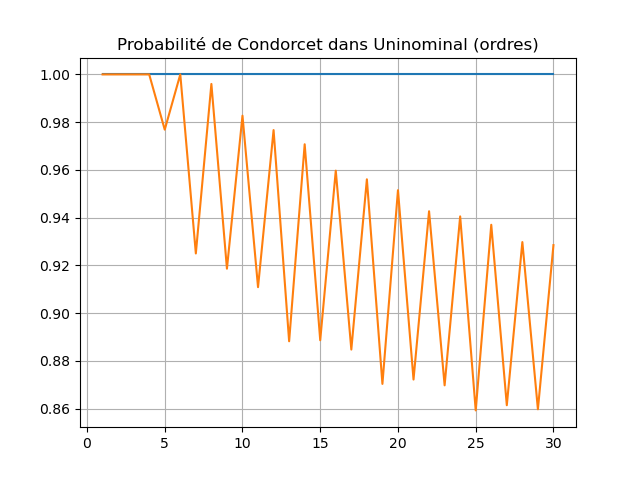
\includegraphics[scale=\sgh]{critereCondorcet/graphe_Uninominal_ordres_3_30.png}
			\hfill
			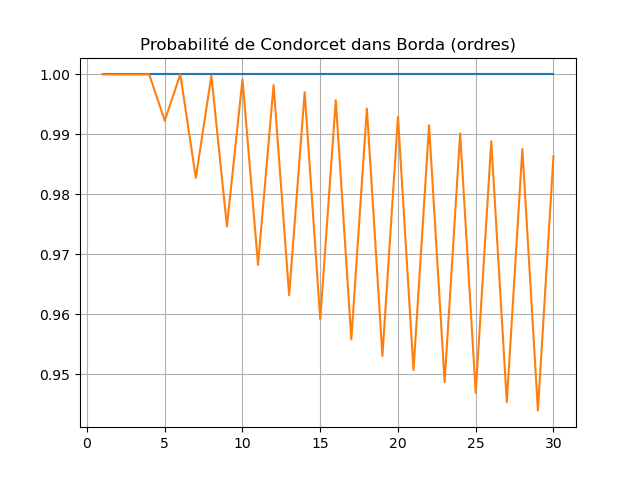
\includegraphics[scale=\sgh]{critereCondorcet/graphe_Borda_ordres_3_30.png}
		\end{subfigure}
	\end{adjustwidth}
\end{figure}

\begin{figure}[H]
	\underline{Critère d'unicité du vainqueur}
	\begin{adjustwidth}{-1cm}{-1cm}
		\centering
		\begin{subfigure}{1\linewidth}
			
\includegraphics[scale=\sgh]{unique_vainqueur/graphe_Uninominal_ordres_3_30.png}
			\hfill
			
\includegraphics[scale=\sgh]{unique_vainqueur/graphe_Borda_ordres_3_30.png}
		\end{subfigure}
	\end{adjustwidth}
\end{figure}
\vspace{-1cm}
\begin{figure}[H]
	\begin{adjustwidth}{-1cm}{-1cm}
		\centering
		\begin{subfigure}{1\linewidth}
			
\includegraphics[scale=\sgh]{unique_vainqueur/graphe_Black_ordres_3_30.png}
			\hfill
			
\includegraphics[scale=\sgh]{unique_vainqueur/graphe_Copeland_ordres_3_30.png}
		\end{subfigure}
	\end{adjustwidth}
\end{figure}
\vspace{-1cm}
\begin{figure}[H]
	\begin{adjustwidth}{-1cm}{-1cm}
		\begin{subfigure}{1\linewidth}
			
\includegraphics[scale=\sgh]{unique_vainqueur/graphe_Schulze_ordres_3_20.png}
		\end{subfigure}
	\end{adjustwidth}
\end{figure}

\begin{figure}[H]
	\underline{Critère de particpation} \\
	La probabilité de ce critère vaut 1 pour les votes pondérés d'après \hyperref[Vote pondéré croissant]{le théorème des votes pondérés croissants}.
	\begin{adjustwidth}{-1cm}{-1cm}
		\centering
		\begin{subfigure}{1\linewidth}
			
\includegraphics[scale=\sgh]{participation/graphe_Black_ordres_3_30.png}
			\hfill
			
\includegraphics[scale=\sgh]{participation/graphe_Copeland_ordres_3_30.png}
		\end{subfigure}
	\end{adjustwidth}
\end{figure}
\vspace{-1cm}
\begin{figure}[H]
	\begin{adjustwidth}{-1cm}{-1cm}
		\begin{subfigure}{1\linewidth}
			
\includegraphics[scale=\sgh]{participation/graphe_Schulze_ordres_3_20.png}
		\end{subfigure}
	\end{adjustwidth}
\end{figure}

\begin{figure}[H]
	\underline{Avec plus de trois candidats} \\
	\begin{adjustwidth}{-1cm}{-1cm}
		\centering
		\begin{subfigure}{1\linewidth}
			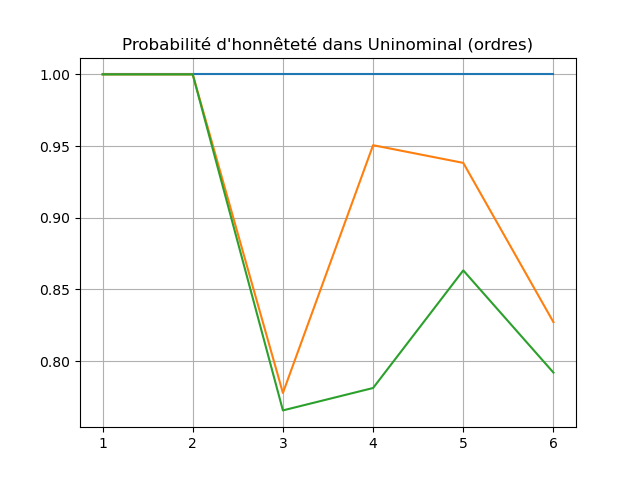
\includegraphics[scale=\sgh]{honnetete/graphe_Uninominal_ordres_4_6.png}
			\hfill
			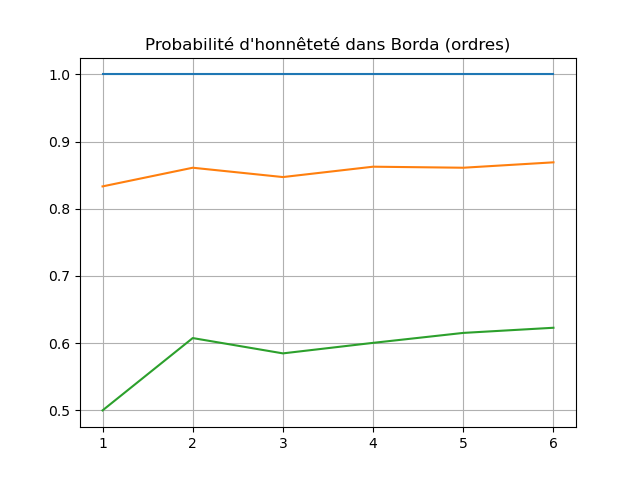
\includegraphics[scale=\sgh]{honnetete/graphe_Borda_ordres_4_6.png}
		\end{subfigure}
	\end{adjustwidth}
\end{figure}
\vspace{-1cm}
\begin{figure}[H]
	\begin{adjustwidth}{-1cm}{-1cm}
		\centering
		\begin{subfigure}{1\linewidth}
			
\includegraphics[scale=\sgh]{honnetete/graphe_Black_ordres_4_6.png}
			\hfill
			
\includegraphics[scale=\sgh]{honnetete/graphe_Copeland_ordres_4_6.png}
		\end{subfigure}
	\end{adjustwidth}
\end{figure}
\vspace{-1cm}
\begin{figure}[H]
	\begin{adjustwidth}{-1cm}{-1cm}
		\begin{subfigure}{1\linewidth}
			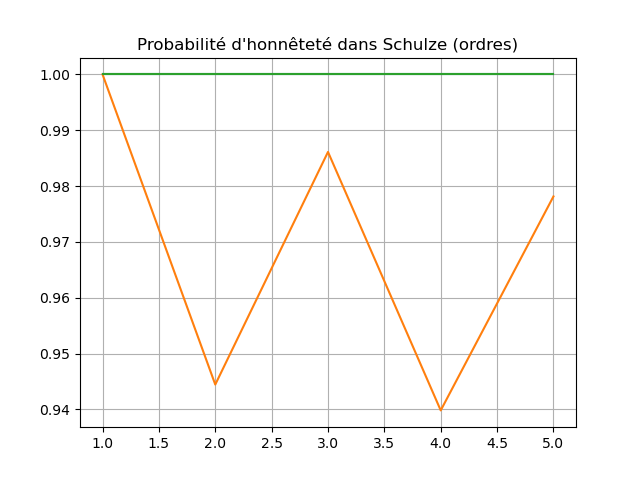
\includegraphics[scale=\sgh]{honnetete/graphe_Schulze_ordres_4_5.png}
		\end{subfigure}
	\end{adjustwidth}
\end{figure}

\begin{figure}[H]
	\begin{adjustwidth}{-1cm}{-1cm}
		\centering
		\begin{subfigure}{1\linewidth}
			
\includegraphics[scale=\sgh]{unique_vainqueur/graphe_Uninominal_ordres_4_7.png}
			\hfill
			
\includegraphics[scale=\sgh]{unique_vainqueur/graphe_Borda_ordres_4_7.png}
		\end{subfigure}
	\end{adjustwidth}
\end{figure}
\begin{figure}[H]
	\begin{adjustwidth}{-1cm}{-1cm}
		\centering
		\begin{subfigure}{1\linewidth}
			
\includegraphics[scale=\sgh]{unique_vainqueur/graphe_Black_ordres_4_6.png}
			\hfill
			
\includegraphics[scale=\sgh]{unique_vainqueur/graphe_Copeland_ordres_4_6.png}
		\end{subfigure}
	\end{adjustwidth}
\end{figure}

\begin{figure}[H]
	\underline{Avec de relations de préordre} \\
	Maintenant, $\D = \pO$.
	\begin{adjustwidth}{-1cm}{-1cm}
		\centering
		\begin{subfigure}{1\linewidth}
			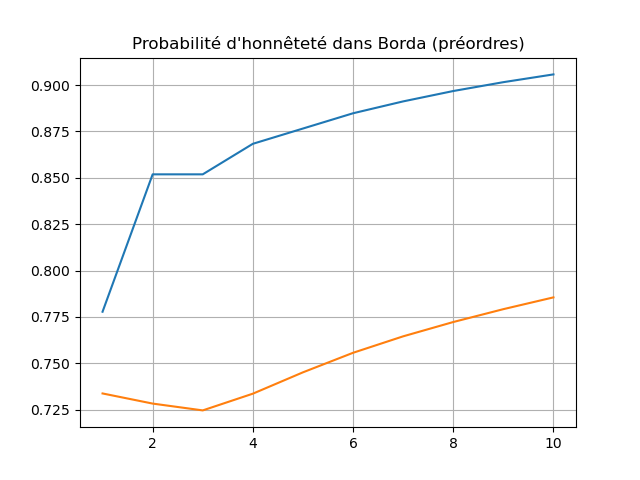
\includegraphics[scale=\sgh]{honnetete/graphe_Borda_préordres_3_10.png}
			\hfill
			
\includegraphics[scale=\sgh]{honnetete/graphe_Black_préordres_3_9.png}
		\end{subfigure}
	\end{adjustwidth}
\end{figure}
\vspace{-1cm}
\begin{figure}[H]
	\begin{adjustwidth}{-1cm}{-1cm}
		\centering
		\begin{subfigure}{1\linewidth}
			
\includegraphics[scale=\sgh]{honnetete/graphe_Copeland_préordres_3_9.png}
			\hfill
			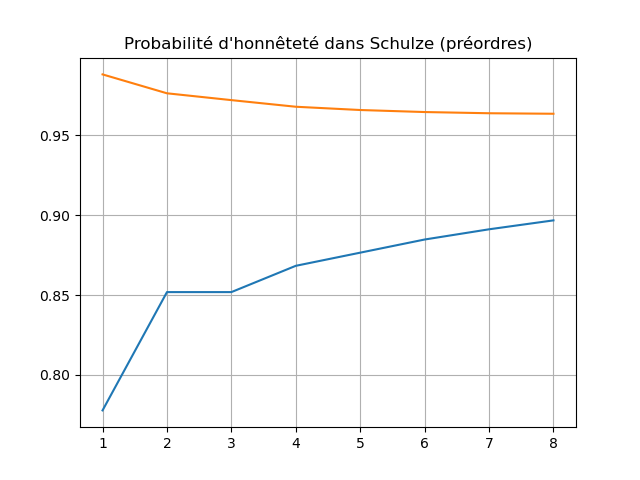
\includegraphics[scale=\sgh]{honnetete/graphe_Schulze_préordres_3_8.png}
		\end{subfigure}
	\end{adjustwidth}
\end{figure}

\begin{figure}[H]
	\begin{adjustwidth}{-1cm}{-1cm}
		\centering
		\begin{subfigure}{1\linewidth}
			
\includegraphics[scale=\sgh]{unique_vainqueur/graphe_Borda_préordres_3_10.png}
			\hfill
			
\includegraphics[scale=\sgh]{unique_vainqueur/graphe_Black_préordres_3_9.png}
		\end{subfigure}
	\end{adjustwidth}
\end{figure}
\vspace{-1cm}
\begin{figure}[H]
	\begin{adjustwidth}{-1cm}{-1cm}
		\centering
		\begin{subfigure}{1\linewidth}
			
\includegraphics[scale=\sgh]{unique_vainqueur/graphe_Copeland_préordres_3_9.png}
			\hfill
			
\includegraphics[scale=\sgh]{unique_vainqueur/graphe_Schulze_préordres_3_8.png}
		\end{subfigure}
	\end{adjustwidth}
\end{figure}

\begin{figure}[H]
	\begin{adjustwidth}{-1cm}{-1cm}
		\centering
		\begin{subfigure}{1\linewidth}
			
\includegraphics[scale=\sgh]{participation/graphe_Black_préordres_3_9.png}
			\hfill
			
\includegraphics[scale=\sgh]{participation/graphe_Copeland_préordres_3_9.png}
		\end{subfigure}
	\end{adjustwidth}
\end{figure}
\vspace{-1cm}
\begin{figure}[H]
	\begin{adjustwidth}{-1cm}{-1cm}
		\begin{subfigure}{1\linewidth}
			
\includegraphics[scale=\sgh]{participation/graphe_Schulze_préordres_3_10.png}
		\end{subfigure}
	\end{adjustwidth}
\end{figure}

\begin{figure}[H]
	\underline{Vote par approbation} \\
	Ici, $\D = \{ \theta \in \pO \;|\; \left| \varXi_\theta(\C) \right| \leqslant 2 \}$.
	Le vote par approbation respecte le critère de participation et celui de Condorcet.
	\begin{adjustwidth}{-1cm}{-1cm}
		\centering
		\begin{subfigure}{1\linewidth}
			
\includegraphics[scale=\sgh]{honnetete/graphe_Approbation_préordresduals_3_20.png}
			\hfill
			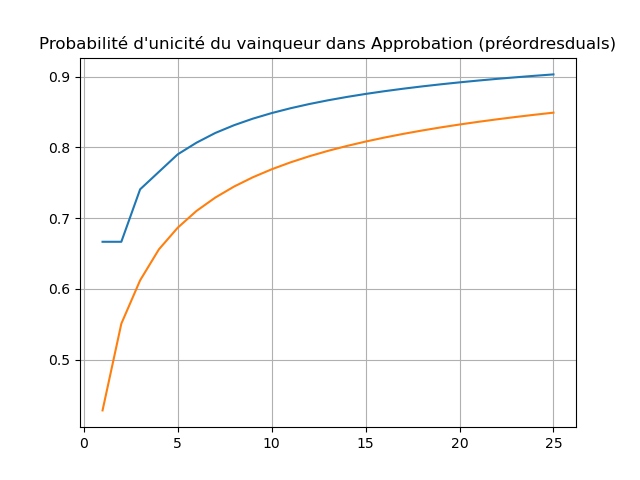
\includegraphics[scale=\sgh]{unique_vainqueur/graphe_Approbation_préordresduals_3_25.png}
		\end{subfigure}
	\end{adjustwidth}
\end{figure}
\vspace{-1cm}
\begin{figure}[H]
	\begin{adjustwidth}{-1cm}{-1cm}
		\centering
		\begin{subfigure}{1\linewidth}
			
\includegraphics[scale=\sgh]{honnetete/graphe_Approbation_préordresduals_5_5.png}
			\hfill
			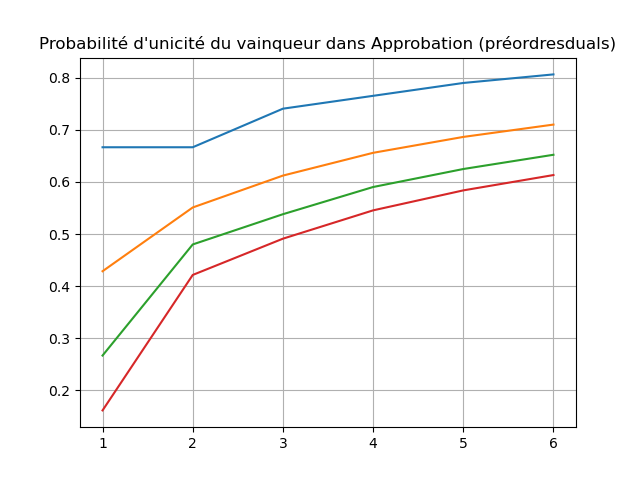
\includegraphics[scale=\sgh]{unique_vainqueur/graphe_Approbation_préordresduals_5_6.png}
		\end{subfigure}
	\end{adjustwidth}
\end{figure}
\vspace{-1cm}
\begin{figure}[H]
	\noindent Dans le même domaine de vote, pour deux autres systèmes de vote :
	\begin{adjustwidth}{-1cm}{-1cm}
		\centering
		\begin{subfigure}{1\linewidth}
			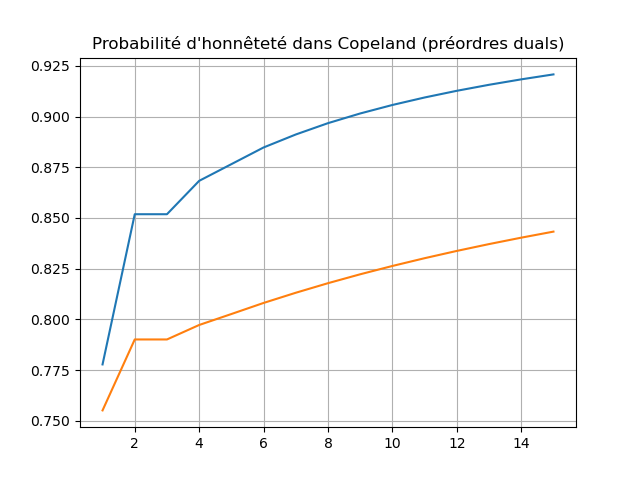
\includegraphics[scale=\sgh]{honnetete/graphe_Copeland_préordresduals_3_15.png}
			\hfill
			
\includegraphics[scale=\sgh]{honnetete/graphe_Schulze_préordresduals_3_10.png}
		\end{subfigure}
	\end{adjustwidth}
\end{figure}

	% !TeX root = TIPE_vangi.tex
% !TeX spellcheck = fr

\section{Conclusion}

Nous avons travaillé sur les relations de préordres pour finalement définir un relation induite sur les relations de préordres. Ainsi, nous avons pu comparé les résultats d'un vote du point de vue d'un électeur quelconque. Ce qui nous a permis de savoir s'il est intéressant pour cet électeur d'être honnête ou de participer.

\textit{La méthode Borda} possède toujours une probabilité inférieure aux autres systèmes de vote (excepté pour l'unicité du vainqueur). C'est le pire système.
\textit{La méthode Black}, par le simple ajout de la recherche de l'existence d'un vainqueur de Condorcet, augment considérablement l'honnêteté qui devient meilleure que celle du \textit{scrutin uninominal}. Elle se comporte plutôt bien lors de l'ajout de choix et sur les préordres, mieux que \textit{La méthode de Copeland}.

\textit{La méthode de Copeland} et \textit{la méthode de Schulze} possédent les meilleures probabilités et respectent le critères de Condorcet : ce qui fait d'elles, les meilleurs systèmes parmi ceux étudiés. De plus, elles ont la même complexité temporelle $O(|\V|^2)$. Certes \textit{la méthode de Copeland} se distingue en ayant plus souvent un unique vainqueur mais \textit{la méthode de Schulze} possède un meilleur comportement vis-à-vis de l'ajout d'un candidat et des préférences décrites comme des préordres.

En plus de permettre aux électeurs une meilleur expression de leur opinion, les relations de préordres ont des courbes plus "lisses" que celles des relations d'ordres. D'ailleurs les axiomes de Von Neumann–Morgenstern posent que les opinions sont des relations de préordres. Ainsi, elles semblent plus naturelles et mieux décrire les opinions individuelles. Mais leurs courbes sont en-dessous de celles des relations d'ordre pour la probabilité d'honnêteté.

\bigbreak\bigbreak

\textbf{À faire} \\
Finir les preuves. \\
Commenter les graphiques et choisir les plus pertinents pour enlever les autres. \\
Expliquer en quoi le critère d'honnêteté est le plus important. \\
Calculer la complexité de l'algorithme. \\

\textbf{Pistes à creuser} \\
Étendre le calcul de la probabilité au vote par meilleur médiane (et aux systèmes de vote aléatoires). \\
Trouver un lien entre critère individuels et collectif. \\
Effectuer un travail empirique \\
Calculer littéralement la probabilité pour des systèmes et des critères simples.

	\addcontentsline{toc}{section}{Références}
	\bibliographystyle{plain}
	\bibliography{articles}
\end{document}